%; whizzy paragraph -pdf xpdf -latex ./whizzypdfptex.sh
%; whizzy-paragraph "^\\\\begin{frame}"
% latex beamer presentation.
% platex, latex-beamer でコンパイルすることを想定。 

%     Tokyo Debian Meeting resources
%     Copyright (C) 2009 Junichi Uekawa
%     Copyright (C) 2009 Nobuhiro Iwamatsu

%     This program is free software; you can redistribute it and/or modify
%     it under the terms of the GNU General Public License as published by
%     the Free Software Foundation; either version 2 of the License, or
%     (at your option) any later version.

%     This program is distributed in the hope that it will be useful,
%     but WITHOUT ANY WARRANTY; without even the implied warreanty of
%     MERCHANTABILITY or FITNESS FOR A PARTICULAR PURPOSE.  See the
%     GNU General Public License for more details.

%     You should have received a copy of the GNU General Public License
%     along with this program; if not, write to the Free Software
%     Foundation, Inc., 51 Franklin St, Fifth Floor, Boston, MA  02110-1301 USA

\documentclass[cjk,dvipdfmx,12pt]{beamer}
\usetheme{Tokyo}
\usepackage{monthlypresentation}
\usepackage{listings}

%  preview (shell-command (concat "evince " (replace-regexp-in-string "tex$" "pdf"(buffer-file-name)) "&")) 
%  presentation (shell-command (concat "xpdf -fullscreen " (replace-regexp-in-string "tex$" "pdf"(buffer-file-name)) "&"))
%  presentation (shell-command (concat "evince " (replace-regexp-in-string "tex$" "pdf"(buffer-file-name)) "&"))

%http://www.naney.org/diki/dk/hyperref.html
%日本語EUC系環境の時
\AtBeginDvi{\special{pdf:tounicode EUC-UCS2}}
%シフトJIS系環境の時
%\AtBeginDvi{\special{pdf:tounicode 90ms-RKSJ-UCS2}}

\title{Golangで書かれたツールを\\Debianパッケージにする}
\subtitle{}
\author{まえだこうへい}
\date{2014年4月19日}
\logo{
\includegraphics[width=8cm]{image200607/openlogo-light.eps}}

\begin{document}
\lstset{ %
  backgroundcolor=\color{dancerlightblue},
  language=sh
}

\frame{\titlepage{}}

\begin{frame}{自己紹介}
 \begin{itemize}
  \item[Debian:] blockdiagシリーズ、django REST framework、\\yrmcdsなどのメンテナ
  \item[言語:] 主にPython。\\最近Golangも使おうと勉強中
  \item[家庭:] 猫一匹(♀)、娘二人、妻一人
  \item[勉強会:] ほぼDebian勉強会のみ。でも今日は約半年ぶり
  \item[仕事:] PythonでLDAPごにょごにょとか、\\django REST frameworkでAPI開発とか
 \end{itemize}
\end{frame}

\begin{frame}{今日の話の流れと前提}
\begin{itemize}
  \item Golangのツールをパッケージ化しようと思った動機
  \item DebianでのGolangを使う方法
  \item Debianパッケージ化に必要なGolangの知識
  \item パッケージ化するためのお作法
  \item GolangのツールをDebianパッケージにする
\end{itemize}

※前提条件: Sidを準備すること
\end{frame}


\begin{frame}{今日の話の流れと前提}
\begin{itemize}
  \item \textcolor{red}{Golangのツールをパッケージ化しようと思った動機}
  \item DebianでのGolangを使う方法
  \item Debianパッケージ化に必要なGolangの知識
  \item パッケージ化するためのお作法
  \item GolangのツールをDebianパッケージにする
\end{itemize}

※前提条件: Sidを準備すること
\end{frame}

\begin{frame}{Serfを使おうと思ったので}
  \begin{itemize}
  \item[0.] やりたいと思っていることをSerfでできそう?
  \item[1.] mainにないのでDebianパッケージを作成すっか
  \item[2.] 依存関係のパッケージも軒並みパッケージ化必要!
  \item[3.] 全部作ったけど多い!pkg-goチームに加入!
  \item[4.] pkg-goのポリシー見たら、パッケージ名など修正必要
  \item[5.] 修正終わったので、ML投稿とITPやるかー←イマココ
  \end{itemize}
\end{frame}

\begin{frame}{Debianパッケージ化が必要なものども(※四角)}
\begin{figure}[H]
\begin{center}
  \includegraphics[width=0.7\hsize]{image201404/serf-dependency.eps}
 \label{fig:serf-dependencies}
\end{center}
\end{figure}
\end{frame}

\begin{frame}{ }
\begin{itemize}
  \item Golangのツールをパッケージ化しようと思った動機
  \item \textcolor{red}{DebianでのGolangを使う方法}
  \item Debianパッケージ化に必要なGolangの知識
  \item パッケージ化するためのお作法
  \item GolangのツールをDebianパッケージにする
\end{itemize}
\end{frame}

\begin{frame}[containsverbatim]{DebianでのGolangの環境構築}
\begin{commandline}
$ sudo apt-get install golang
\end{commandline}
\end{frame}

\begin{frame}{インストールされるパッケージ}
\begin{itemize}
\item golang-doc
\item golang-go
\item golang-go-linux-amd64 \footnote{amd64の場合}
\item golang-go.tools
\item golang-src
\item libjs-jquery
\item javascript-common
\end{itemize}
\end{frame}


\begin{frame}{ }
\begin{itemize}
  \item Golangのツールをパッケージ化しようと思った動機
  \item DebianでのGolangを使う方法
  \item \textcolor{red}{Debianパッケージ化に必要なGolangの知識}
  \item パッケージ化するためのお作法
  \item GolangのツールをDebianパッケージにする
\end{itemize}
\end{frame}

\begin{frame}[containsverbatim]{Golangのコンパイル方法}
  hello world(hello.go)を用意
 \begin{commandline}
package main

import "fmt"

func main() {
  fmt.Println("Hello world.")
}
 \end{commandline}
\end{frame}

\begin{frame}[containsverbatim]{Golangのコンパイル方法}
  go buildでコンパイル
 \begin{commandline}
$ go build hello.go
 \end{commandline}
\end{frame}

\begin{frame}[containsverbatim]{Golangのコンパイル方法}
実行
 \begin{commandline}
$ ./hello
Hello world.
 \end{commandline}
\end{frame}

\begin{frame}[containsverbatim]{Golangのコンパイル方法}
静的リンクされていることを確認
 \begin{commandline}
$ file hello
hello: ELF 64-bit LSB executable, x86-64, \
version 1 (SYSV), statically linked, not stripped
 \end{commandline}
\end{frame}

\begin{frame}[containsverbatim]{標準ライブラリ以外に依存する場合}
\begin{itemize}
  \item 環境変数GOPATHを設定
  \item 標準ライブラリ以外のGolangのDebianパッケージは、/usr/share/gocodeにインストールされる
\end{itemize}
\begin{commandline}
$ export GOPATH=/usr/share/gocode
\end{commandline}
\end{frame}

\begin{frame}[containsverbatim]{標準ライブラリ以外に依存する場合}
golang-dns-dev(Go用のDNSライブラリ)を使ってみる
\begin{commandline}
$ sudo apt-get install golang-dns-dev
$ dpkg -L golang-dns-dev
(snip)
/usr/share/gocode
/usr/share/gocode/src
/usr/share/gocode/src/github.com
/usr/share/gocode/src/github.com/miekg
/usr/share/gocode/src/github.com/miekg/dns
/usr/share/gocode/src/github.com/miekg/dns/zscan_rr.go
/usr/share/gocode/src/github.com/miekg/dns/zscan.go
\end{commandline}
\end{frame}

\begin{frame}[containsverbatim]{標準ライブラリ以外に依存する場合}
Golangのツールで依存パッケージをインストール場合
※ユーザディレクトリにインストールする例
\begin{commandline}
$ mkdir $HOME/gocode
$ export GOPATH=$HOME/gocode
$ go get github.com/miekg/dns
\end{commandline}
\end{frame}

\begin{frame}[containsverbatim]{標準ライブラリ以外に依存する場合}

importのみ抜粋\footnote{参照: \url{https://github.com/mkouhei/godig/blob/devel/dig.go}}
\begin{commandline}
package main

import (
"github.com/miekg/dns"
"fmt"
"flag"
)

(snip)
\end{commandline}
\end{frame}

\begin{frame}[containsverbatim]{標準ライブラリ以外に依存する場合}

実行
{\tiny
{\begin{lstlisting}
$ go run dig.go
example.org.    2022    IN      SOA     sns.dns.icann.org. noc.dns.icann.org.\
 2013103528 7200 3600 1209600 3600

$ go run dig.go -d debian.or.jp.
debian.or.jp.   600     IN      SOA     ns.debian.or.jp. root.debian.or.jp.\
 2013091001 600 86400 2419200 1440
\end{lstlisting}}}
\end{frame}

\begin{frame}{ }
\begin{itemize}
  \item Golangのツールをパッケージ化しようと思った動機
  \item DebianでのGolangを使う方法
  \item Debianパッケージ化に必要なGolangの知識
  \item \textcolor{red}{パッケージ化するためのお作法}
  \item GolangのツールをDebianパッケージにする
\end{itemize}
\end{frame}

\begin{frame}{GolangのDebianパッケージ化のお作法}
  バイナリのみの場合
  \begin{itemize}
  \item 基本的にはDependsは必要ない
  \item デーモン化すると必要になるケースもある
  \item パッケージ名はUpstreamの名称と同じでもよい
  \end{itemize}
\end{frame}

\begin{frame}{GolangのDebianパッケージ化のお作法}
  ライブラリのみの場合
  \begin{itemize}
  \item ソースコードの配布だけなのでコンパイルは不要
  \item バイナリと一緒に配布する場合は、バイナリと同様
  \item ソースパッケージ、バイナリパッケージとも"golang-"というprefixが必要
  \item バイナリパッケージには"-dev"というsuffixも必要
  \end{itemize}
\end{frame}

\begin{frame}{GolangのDebianパッケージ化のお作法}
 共通
 \begin{itemize}
 \item ビルドやテスト実行時に、\texttt{go get}を使ってはアカン
 \item 伝統的なバージョンニングがされていなければ"0.0~git20140419-1"というバージョンをつける
 \item ソースパッケージはgit-buildpackageで管理する
\end{itemize}
\end{frame}


\begin{frame}{ }
\begin{itemize}
  \item Golangのツールをパッケージ化しようと思った動機
  \item DebianでのGolangを使う方法
  \item Debianパッケージ化に必要なGolangの知識
  \item パッケージ化するためのお作法
  \item \textcolor{red}{GolangのツールをDebianパッケージにする}
\end{itemize}
\end{frame}

\begin{frame}{ソースコードの入手}
\begin{itemize}
  \item tarballがあればそれをなければ、リポジトリから入手
  \item バージョンを確認する\footnote{なければ前述の0.0~git20140419のようなバージョンをつける}
  \item ソースパッケージ用のGitリポジトリを作り、\texttt{git import-orig}コマンドでインポートする
\end{itemize}
\end{frame}


\begin{frame}{ソースパッケージの作成}
\begin{itemize}
  \item[1.] \texttt{dh\_make}コマンドでdebianディレクトリを生成
  \item[2.] 不要なテンプレートを削除
  \item[3.] control,copyright,rules,changelogなどを修正
  \item[4.] \texttt{git-buildpackage}コマンドでパッケージをビルド\footnote{mainに入っていないパッケージに依存していない場合は、\texttt{pbuilder}の方が個人的には楽}
\end{itemize}
\end{frame}

\begin{frame}{debian/control}
  \begin{itemize}
    \item 共通
      \begin{itemize}
      \item Build-Dependsにgolang-go
      \end{itemize}
    \item ライブラリ
      \begin{itemize}
      \item Build-Dependsにdh-golang
      \item Dependsにgolang-goを追記
      \item Architecture: all
      \end{itemize}
    \item バイナリ
      \begin{itemize}
        \item Architecture: any
      \end{itemize}
  \end{itemize}
\end{frame}

\begin{frame}{debian/rules}
  \begin{itemize}
  \item 共通
    \begin{itemize}
    \item \texttt{dh}コマンドに\texttt{--buildsystem=golang}オプションを指定
    \end{itemize}
  \item ライブラリ
    \begin{itemize}
    \item 環境変数\texttt{DH\_GOPKG}に\texttt{GOPATH}で指定したディレクトリしたに展開される名前空間を指定
    \item \texttt{dh}コマンドに\texttt{--with=golang}オプションを指定
    \item \texttt{override\_dh\_auto\_install}ターゲットで、\texttt{dh\_auto\_install -O-buildsystem=golang}を設定
    \end{itemize}
  \item バイナリ
    \begin{itemize}
      \item \texttt{dh}コマンドに\texttt{--with=golang}オプションが不要
    \end{itemize}
\end{itemize}

\end{frame}

\begin{frame}{まとめ}
\begin{itemize}
  \item Debianパッケージを作る上で必要なGolangパッケージ、コンパイルの方法
  \item GolangのDebainパッケージ化
  \item pkg-go teamによるGolangパッケージのポリシー
\end{itemize}
\end{frame}

\end{document}
